\documentclass [12pt]{article}
\usepackage{graphicx}
\usepackage{amstext,verbatim,alltt}
\usepackage{moreverb}
\setlength{\textwidth}{6.5in}
\setlength{\oddsidemargin}{0in}
\setlength{\evensidemargin}{0in}
\begin{document}

\title{The MPBench Report}
\author {Philip J. Mucci \\
	Kevin London \\
	John Thurman \\
        {\tt mucci@cs.utk.edu} \\
	{\tt london@cs.utk.edu} \\
	{\tt thurman@cs.utk.edu}}

\date{November 1998}

\maketitle

\section{Introduction}

MPBench is a benchmark to evaluate the performance of MPI
on MPP's and clusters of workstations. It uses a flexible
and portable framework to allow benchmarking of any message passing
layer with similar send and receive semantics. It generates two types
of reports, consisting of the raw data files and Postscript
graphs. No interpretation or analysis of the data is performed, it is
left entirely up to the user.

\section{How it works}

MPBench currently tests eight different MPI calls. The following functions are measured.  
The default number of processes used can be set in {\tt make.def}. \\

\begin{center}
\begin{tabular}{|l|l|r|} \hline
{\em Benchmark} & {\em Units } & {\em \# Processes}\\ \hline
Bandwidth & Megabytes/sec  & 2 \\ \hline
Roundtrip & Transactions/sec & 2 \\ \hline
Application Latency & Microseconds & 2 \\ \hline
Broadcast & Megabytes/sec & make.def value \\ \hline
Reduce & Megabytes/sec & make.def value \\ \hline
AllReduce & Megabytes/sec & make.def value \\ \hline
Bidirectional Bandwidth & Megabytes/sec & 2 \\ \hline
All-to-All & Megabytes/sec & make.def value \\ \hline
\end{tabular}
\end{center}

All tests are timed in the following manner.
\begin{enumerate}
\item Set up the test.
\item Start the timer.
\item Loop of operations over the message size as a power of two 
and the iteration count.
\item Verify that those operations have completed.
\item Stop the timer.
\item Compute the appropriate metric.
\end{enumerate}

By default, MPBench measures messages from 4 bytes to $ 2^{16} $ bytes, in 
powers of two for 100 iterations.  Each test is run a single time before testing 
to allow for cache setup and routing.  The cache is then flushed before each repetition 
and before each new message size is tested.  The cache is not flushed however betwen 
iterations on the same message size, which are averaged. 

In MPBench, we avoid calling the timer around every operation, because
this often results in the faulty reporting of data. Some of these
operations on MPP's take so little time, that the accuracy and latency
of accessing the system's clock would significantly affect the
reported data. Thus it is only appropriate that we perform our timing
operations {\em outside the loop}. Some MPP's and workstations have
the capability to access the system's timer registers, but this is not
portable and would introduce unnecessary complexity into the code to
compensate for situations where the timing routines were not
efficient.

For simplicity purposes, we will refer to two different types of tasks in
MPBench, the master of which there is only one, and the slaves of
which their may be any number. The point-to-point tests only use two
tasks, a master and a slave. The other tests run with any number of
slaves, the default being sixteen.

MPBench averages performance over a number of iterations. The user
should be aware that MPBench will use a lower number of iterations
than the one specified for certain situations. This should not effect
the accuracy of the results, as the iteration count is only changed
when the message lengths are prohibitively large. 

It should be noted that cachebench does not dictate the placement of slave
tasks. This can cause the user to make false claims about the performance
of distributed multiprocessors like the Origin 2000. MPBench measures 
point-to-point performance on MPI jobs with 2 tasks. For systems like the
Origin, this means both tasks will be running on the same physical board and
their communication performance will largely be dominated by the speed at
which they can copy memory. The next version of MPBench will include the
ability to measure processors that are logically farther away from the master.

\subsection{Notes on MPI}
There are many different send and receive calls in MPI each with
different semantics for usage and completion. Here we focus on the
{\em default} mode of sending. This means we are not using any
{\em nonblocking} or {\em immediate} communication calls. Each MPI 
implementation handles the default mode a bit differently, but the
algorithm is usually a derivative of the following. 

\begin{verbatim}
send first chunk of message
if message is larger than size N
  wait for reply and destination address Y
    send rest of message directly to address Y
else
  if more to send
    send rest of message
endif
\end{verbatim}

MPI does this to
avoid unnecessary copies of the data, which usually dominates the
cost of any communication layer. The receiving process will 
buffer a limited amount of data before informing the sender of
the destination address in the application. This way, a large message is
received directly into the application's data structure rather than
being held in temporary storage like with PVM. The problem with this is
that for large messages, {\tt sends} cannot complete before their
corresponding {\tt receives}. This introduces possibly synchronization
and portability problems.

\subsection{Bandwidth}

MPBench measures bandwidth with a doubly nested loop. The outer loop
varies the message size, and the inner loop measures the send operation
over the iteration count. After the iteration count is reached, the
slave process {\em acknowledges} the data it has received by sending a four
byte message back to the master. This informs the sender when the
slaves have completely finished receiving their data and are ready to
proceed. This is necessary, because the send on the master may
complete before the matching receive does on the slave. This exchange
does introduce additional overhead, but given a large iteration count,
its effect is minimal. \\

The master's pseudo code for this test is as follows:
\begin{verbatim}
do over all message sizes
  start timer
  do over iteration count
    send(message size)
  recv(4)
  stop timer
\end{verbatim}

The slaves' pseudo code is as follows:
\begin{verbatim}
do over all message sizes
  start timer
  do over iteration count
    recv(message size)
  send(4)
  stop timer
\end{verbatim}

\subsection{Bidirectional Bandwidth}

MPBench measures bidirectional bandwidth with a doubly nested loop. The outer loop
varies the message size, and the inner loop measures the send operation
over the iteration count.  Both processes execute a non-blocking receive, then a non-blocking 
send, and then a wait for each iteration.  The next iteration is prevented from proceeding until
the previous one is finished by the MPI\_Waitall() call, which will not allow execution to 
continue until both messages have been completed. \\

The code for this test is as follows:
\begin{verbatim}
do over all message sizes
  start timer
  do over iteration count
    immediate (nonblocking) receive(message size)	
    immediate (nonblocking) send(message size)
    wait until messages on both ends have been received	
  stop timer
\end{verbatim}

\subsection{Roundtrip}

Roundtrip times are measured in much the same way as bandwidth, except
that, the slave process, after receiving the message, echoes it
back to the master. This benchmark is often referred to as {\em
ping-pong}. Here our metric is transactions per second, which is a
common metric for database and server applications. No acknowledgment
is needed with this test as it is implicit given its semantics. \\
\newpage
The master's pseudo code for this test is as follows:
\begin{verbatim}
do over all message sizes
  start timer
  do over iteration count
    send(message size)
    recv(message size)
  stop timer
\end{verbatim}

The slaves' pseudo code is as follows:
\begin{verbatim}
do over all message sizes
  start timer
  do over iteration count
    recv(message size)
    send(message size)
  stop timer
\end{verbatim}

\subsection{Application Latency}

Application latency is something relatively unique to MPBench. This
benchmark can properly be described as one that measures the time for
an application to issue a {\tt send} and continue computing. The
results for this test vary greatly given how the message passing layer
is implemented. For example, PVM will buffer all messages for
transmission, regardless of whether or not the remote node is ready to
receive the data. MPI on the other hand, will not buffer messages over
a certain size, and thus will block until the remote process has
executed some form of a {\tt receive}. This benchmark is the same as
bandwidth except that we do not acknowledge the data and we report our
results in units of time. \\

The master's pseudo code for this test is as follows:
\begin{verbatim}
do over all message sizes
  start timer
  do over iteration count
    send(message size)
  stop timer
\end{verbatim}

The slaves' pseudo code is as follows:
\begin{verbatim}
do over all message sizes
  start timer
  do over iteration count
    recv(message size)
  stop timer
\end{verbatim}

\subsection{Broadcast and Reduce}

The two functions are also very heavily used in many parallel
applications. Essentially these operations are mirror images of one
another, the different being that reduce reveres the direction of 
communication and performs some computation with the data during
intermediate steps. Both of these benchmarks return the number of
megabytes per second computed from the iteration count and the length
argument given to function call.  \\

Here is the pseudo code for both the master and the slave:
\begin{verbatim}
do over all message sizes
  start timer
  do over iteration count
    reduce or broadcast(message size)
  stop timer
\end{verbatim}

\subsection{AllReduce}

AllReduce is a derivative of an all-to-all communication, where every
process has data for every other. While this operation could easily be
implemented with a reduce followed by a broadcast, that would be highly
inefficient for large message sizes. The PVM version of this test
does this exactly, plus an additional barrier call.
The goal of including this benchmark
is to spot poor implementations so that the application engineer might
be able to restructure his communication. \\

Here is the pseudo code for both the master and the slave:
\begin{verbatim}
do over all message sizes
  start timer
  do over iteration count
    allreduce(message size)
  stop timer
\end{verbatim}

\subsection{All-to-all}

MPBench measures a kind of round-robin communication among multiple processes. The outer loop
varies the message size, and the inner loop measures the send operation over the iteration count. 
Each process sends a message of the size of the total message size divided by the number of processes to 
every other process.  \\

The code for this test is as follows:
\begin{verbatim}
do over all message sizes
  start timer
  do over iteration count
    all-to-all(message size)
  stop timer
\end{verbatim}

\section{Using MPBench}

\subsection{Obtain the Distribution}
MPBench is now found in the LLCbench distribution.
The latest release of LLCbench can always be found through the original author's homepage at \\
{\tt http://www.cs.utk.edu/$\sim$mucci} \\ at its home page at \\ 
{\tt http://www.cs.utk.edu/$\sim$thurman/llcbench} \\
or via FTP at \\ {\tt ftp://cs.utk.edu/~thurman/pub/llcbench.tar.gz}.\\

Now unpack the installation using {\tt gzip} and {\tt tar}.

\begin{verbatim}
kiwi> gzip -dc llcbench.tar.gz | tar xvf -
kiwi> cd llcbench
kiwi>  ls
Makefile     cachebench/  index.html   mpbench/     sys.def@
blasbench/   conf/        make.def     pix/

\end{verbatim}

\subsection{Build the Distribution}

First we must configure the build for our machine, OS and MPI libraries. All
configurations support the reference MPI if available. Before configuration 
{\tt make} with no arguments lists the possible targets.

\begin{verbatim}
kiwi> make
Please use one of the following targets:

        solaris sunos5
        sun sunos4
        sgi-o2k o2k
        linux-mpich
        linux-lam
        alpha
        t3e
        ppc ibm-ppc
        pow2 ibm-pow2
        reconfig (to bring this menu up again)

\end{verbatim}

Configure the build. Here, we are on a Solaris workstation.

\begin{verbatim}
kiwi> make solaris
ln -s conf/sys.solaris sys.def

\end{verbatim}

MPBench's default runtime variable values are contained in the file {\tt make.def} and may
be modified there.  Also examine the {\tt sys.def} file to ensure proper compiler flags and paths to
the MPI libraries.  \\

Now type make to get options for building a benchmark.

\begin{verbatim}
kiwi> make
Please use one of the following targets:

For all three : bench, run, graphs
For Blasbench : blas-bench, blas-run, blas-graphs
For Cachebench: cache-bench, cache-run, cache-graphs
For MPbench   : mp-bench, mp-run mp-graphs

kiwi> make mp-bench
cd mpbench; make mpi_bench
cc -fast -I/src/icl/MPI/mpich/include -DMPI -c mpbench.c -o mpbench.o
cc -fast mpbench.o -o mpi_bench -L/src/icl/MPI/mpich/lib/solaris/ch_p4 -lmpi -lsocket -lnsl 

\end{verbatim}

\subsection{Running MPBench}

While MPBench can be run from the command line, it is designed to be run
from via the {\tt Makefile}.  Running it via the makefile automates the collection and
presentation process. By default, the makefile runs
with the arguments {\tt  -e 1 -i 100 -x 2 -m 16} and with 16 processes. This says that each 
size should be repeated only once, the iteration count should be
set to 100, two measurements are taken betwen every problem size value that is a power of two, 
and the maximum problem size tested is $2 ^{16}$ bytes. You can change the default settings 
by changing the variables in the {\tt make.def} after you have configured the distribution.

When running MPI, sometimes it is required that
you set up a hostfile containing the names of the hosts on which to run the 
processes. If your installation requires a hostfile, MPBench will tell you. 
If that happens, please check your {\tt mpirun} man page for the format.
The resulting datafiles for each of the runs will be left in \\
{\tt mpbench/results/<OS>-<HOSTNAME>\_<API>\_<test>.dat}.



\begin{verbatim}

kiwi> make mp-run
cd mpbench; make run
 Latency test...
 Roundtrip test...
 Bandwidth test...
 Bidirectional Bandwidth test...
 Broadcast test...
 Reduce test...
 Allreduce test...
 All-to-all test...

Datafiles are located in the mpbench/results directory.

\end{verbatim}

Now we plot the results with GNUplot. If GNUplot is not available on
your system, perform the following.

\begin{itemize}
\item Unpack the distribution on a machine that does.
\item Copy your results files to the new machine in the MPBench directory.
\item Execute make\_graphs.sh with the common prefix of your datafiles.
\end{itemize}

Normally, we can make the graphs immediately.

\begin{verbatim}

kiwi> make mp-graphs
cd mpbench; make graphs
results/SunOS-kiwi_mpi
Graphing results/SunOS-kiwi_mpi_latency.dat...
Postscript graph is in results/SunOS-kiwi_mpi_latency.ps.
Graphing results/SunOS-kiwi_mpi_roundtrip.dat...
Postscript graph is in results/SunOS-kiwi_mpi_roundtrip.ps.
Graphing results/SunOS-kiwi_mpi_bandwidth.dat...
Postscript graph is in results/SunOS-kiwi_mpi_bandwidth.ps.
Graphing results/SunOS-kiwi_mpi_bibandwidth.dat...
Postscript graph is in results/SunOS-kiwi_mpi_bibandwidth.ps.
Graphing results/SunOS-kiwi_mpi_alltoall.dat...
Postscript graph is in results/SunOS-kiwi_mpi_alltoall.ps.
Graphing results/SunOS-kiwi_mpi_broadcast.dat...
Postscript graph is in results/SunOS-kiwi_mpi_broadcast.ps.
Graphing results/SunOS-kiwi_mpi_reduce.dat...
Postscript graph is in results/SunOS-kiwi_mpi_reduce.ps.
Graphing results/SunOS-kiwi_mpi_allreduce.dat...
Postscript graph is in results/SunOS-kiwi_mpi_allreduce.ps.

Graphs are located in the mpbench/results directory.

\end{verbatim}

The graphs will be left in the {\tt results} directory.

\section {Usage}

\begin{verbatim}
Usage: (MPI implementation dependent portion) mpi_bench -blracyz [-i #] [-x #] [-m #] [-d #] [-e #]
         -b Do bandwidth benchmark
         -d Do bidirectional bandwidth benchmark
         -l Do latency benchmark
         -r Do roundtrip benchmark
         -a Do all-to-all benchmark
         -c Do broadcast benchmark
         -y Do reduce benchmark
         -z Do allreduce benchmark
         -i Specify the iterations over which to average. 
         -x Specify the number of measurements between powers of 2.  
         -m Specify the log2(available physical memory) to be used 
            as the maximum message size.
         -e Specify the repeat count per message size. 
\end{verbatim}

\newpage
\section{Results on the CEWES MSRC Machines}

The following section contains the graphs of each of the following machines.

\subsection{Latency}
\begin{figure}[Hht]
\centerline{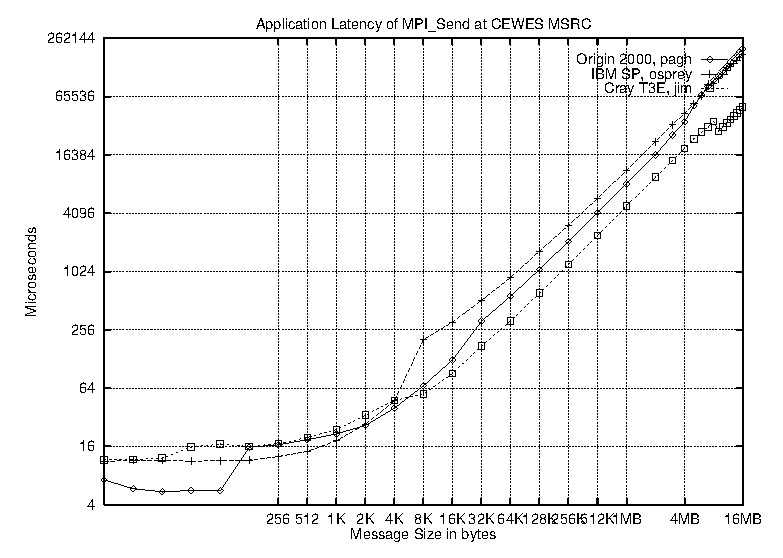
\includegraphics{pics/cewes_mpi_latency.ps}}
\caption{Application Latency of Send}\label{latency}
\end{figure}

In the figure \ref{latency} we see three interesting performance
variations. First note the jump in latency of the T3E when the message
is greater than 64 bytes. This is likely due to space allocated in the
header exchanged between two processes. Many message passing systems
allocate space in the header for a small payload so only one exchange
is required. Next we note the jump in latency on the SP for messages
larger than 4096 bytes. This is the point where IBM's MPI switches to
a rendezvous protocol. This is tunable from the command line for {\tt
poe} IBM's version of {\tt mpirun} with the {\tt -eagerlimit}
argument. It is also tunable with the {\tt MP\_EAGERLIMIT} environment
variable. We recommend setting this to 16384 bytes for all runs. In
fact, IBM does this when running parallel benchmarks. Lastly we note
the falloff in performance at 8MB on the T3E. This is found throughout
all our communication graphs and we are unable to explain it.

\clearpage
\newpage

\subsection{Roundtrip}
\begin{figure}[Hht]
\centerline{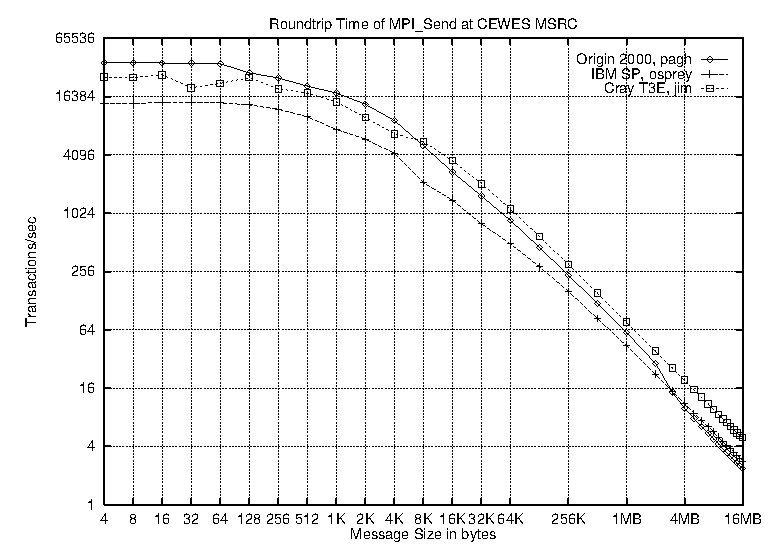
\includegraphics{pics/cewes_mpi_roundtrip.ps}}
\caption{Roundtrip Time of Ping-Pong}\label{roundtrip}
\end{figure}

For small messages, roundtrip time is largely dominated by protocol
overheads and the means to access the network. Notice in figure \ref{roundtrip} that while both
the link speed and the clock speed for the T3E is higher than the Origin,
the Origin still outperforms both machines quite significantly. An inversion
takes place at 8K messages between the Origin and the T3E. We conclude that 
the Origin with its distributed shared memory hardware provides a very
lightweight method of accessing remote memory. 8K is the page size of the
Origin 2000, so it is not surprising that a penalty is paid after crossing
that boundary. At larger messages, the raw link speed of the T3E clearly
dominates, while the performance of the SP and the Origin falters.

\clearpage
\newpage

\subsection{Bandwidth}
\begin{figure}[Hht]
\centerline{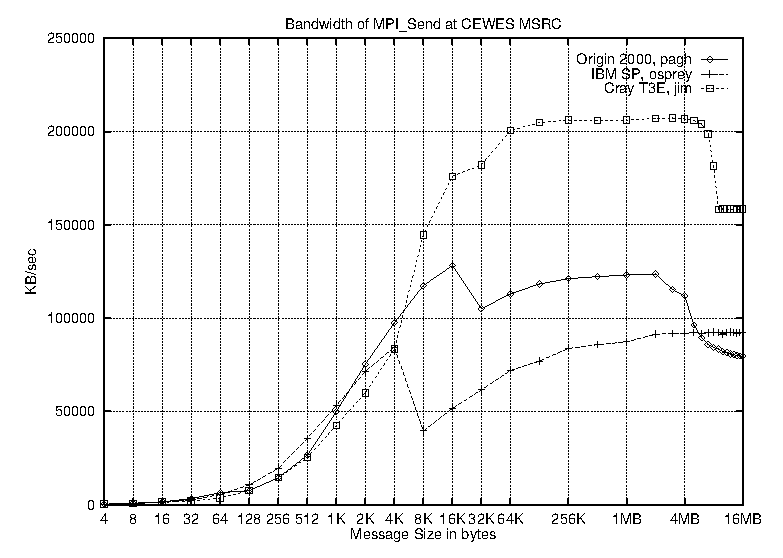
\includegraphics{pics/cewes_mpi_bandwidth.ps}}
\caption{Bandwidth of Send}\label{bandwidth}
\end{figure}

In figure \ref{bandwidth}, we note the dramatic effect of MPI's rendezvous protocol. As mentioned,
the SP has a rather small limit of 4K, thus responsible for the falloff at
larger message sizes. The Origin and the T3E both have an eager limit set
to 16K, with only the Origin suffering a loss in performance at larger sizes.
Also of interest is the effect that caching has on the Origin. As mentioned,
these tests are repeated a number of times, so most of the data will lie
in the Origin's large 4MB level two cache. Note that for larger sizes,
its performance suffers severely.

\clearpage
\newpage

\subsection{Broadcast}
\begin{figure}[Hht]
\centerline{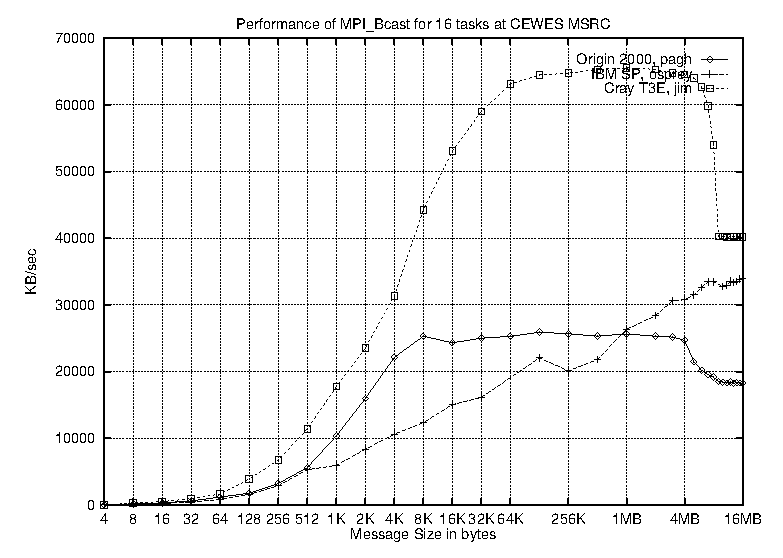
\includegraphics{pics/cewes_mpi_broadcast.ps}}
\caption{Broadcast Performance}\label{broadcast}
\end{figure}

For figure \ref{broadcast}, we again note the dramatic drop-off found at the 8MB message
size on the T3E. For the Origin, we also notice the effect of cache. The user
should be aware that this test also includes the time for an acknowledge to
be sent back to the master. Thus for 16 nodes, and assuming a binary tree
distribution algorithm, we must wait for at least {\tt log2(16) } or 4
sends to complete before we receive our first acknowledgment. 

\clearpage
\newpage

\subsection{Reduce}
\begin{figure}[Hht]
\centerline{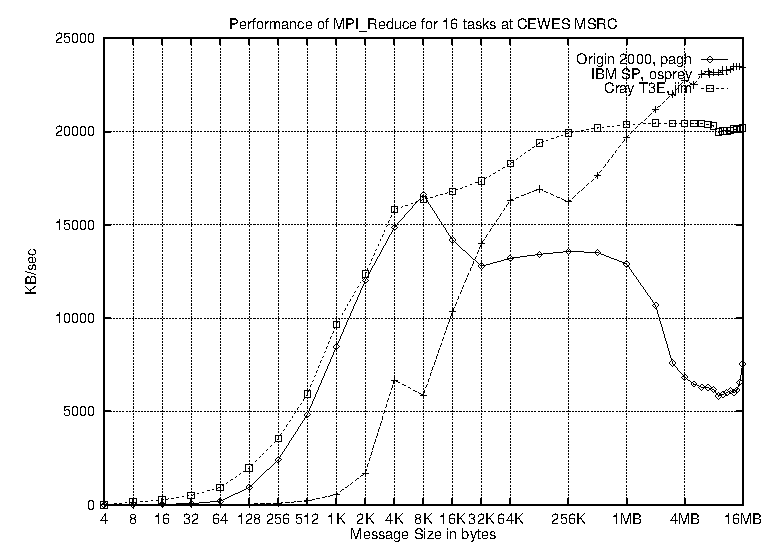
\includegraphics{pics/cewes_mpi_reduce.ps}}
\caption{Reduce Performance}\label{reduce}
\end{figure}

In figure \ref{reduce} we see the effects of cache and shared page size on the Origin. 
For the SP, the dip at the 4K message size is again related to the rather
small eager limit. It is clear that MPI\_Reduce on the SP is implemented
in terms of MPI\_Send at a lower level. Performance of the T3E increases
steadily and levels off around 20MB/sec. Notice the lack of a significant
falloff at larger messages on the T3E. Also notice how poorly the T3E performs
in relation to figure \ref{broadcast}.

\clearpage
\newpage

\subsection{AllReduce}
\begin{figure}[Hht]
\centerline{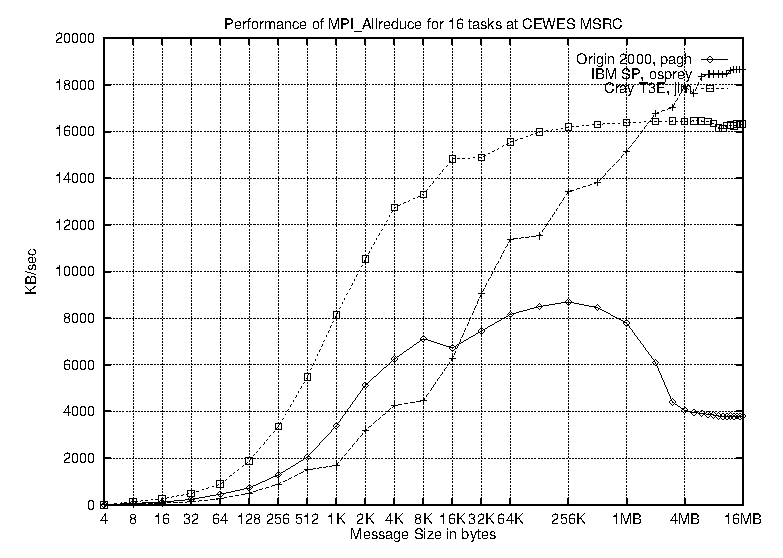
\includegraphics{pics/cewes_mpi_allreduce.ps}}
\caption{AllReduce Performance}\label{allreduce}
\end{figure}

For figure \ref{allreduce}, we again notice the dramatic effect caching has on the
Origin with performance falling off around the 4MB mark. Comparing this
graph with that of figure \ref{reduce}, we note that the SP2 and the T3E
perform about twenty percent worse on Allreduce than on Reduce. The Origin
performs more than thirty percent worse, which is perhaps an architectural
problem related to network contention. 

\section{References}

{\em PVM - Parallel Virtual Machine} Al Geist, Adam Beguelin, Jack Dongarra, Weicheng Jiang, Robert Manchek, Vaidy Sunderam, MIT Press, 1994 \ \\ \ \\
{\em MPI - The Complete Reference} Marc Snir, Steve W. Otto, Steve Huss-Lederman, David W. Walker, Jack Dongarra, MIT Press, 1996

\end{document}
